\subsection{LOCALLY COMPACT SPACES}

DEFINITION 4. A topological space X is said to be locally compact if it is Hausdorff and if every point of X has a compact neighbourhood.

Clearly a compact space is locally compact, but the converse is false; for example, every discrete space is locally compact, but not compact if infinite.

* As we shall see in Chapter IV, § 2, the real line R is locally compact, but not compact. *

PROPOSITION 9. Every locally compact space is regular.

Let X be a locally compact space, then every point \(x \in X\) has a compact neighbourhood V; since X is Hausdorff, V is closed (no. 3, Proposition 4). On the other hand, V is a regular subspace of X (no. 2, Corollary to Proposition 1) and therefore X is regular (§ 8, no. 4, Proposition 13).

COROLLARY. In a locally compact space every point has a fundamental system of compact neighbourhoods.

For the intersection of a closed neighbourhood of x and a compact neighbourhood of x is a compact neighbourhood of x (no. 3, Proposition 3).

\pandocbounded{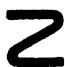
\includegraphics[keepaspectratio]{images/part001_13daf5c9.jpg}}

There exist non-Hausdorff topological spaces in which every point has a fundamental system of compact neighbourhoods (Exercise 5).

The Corollary to Proposition 9 may be generalized as follows:

PROPOSITION 10. In a locally compact space X, every compact set K has a fundamental system of compact neighbourhoods.

Let \(\mathbf{U}\) be any neighbourhood of \(\mathbf{K}\) . For each \(x \in \mathbf{K}\) there is a compact neighbourhood \(\mathbf{W}(x)\) of \(x\) contained in \(\mathbf{U}\) . The interiors of the sets

W (x) form an open covering of K as x runs through K; hence there exist a finite number of points \(x_{i} \in K\) ( \(1 \leqslant i \leqslant n\) ) such that the interiors of the \(W(x_{i})\) cover K. The union V of the \(W(x_{i})\) is therefore a compact neighbourhood of K contained in U (no. 3, Proposition 5).

PROPOSITION 11. Let X be a locally compact space and F a subset of X such that \(F \cap K\) is compact whenever K is a compact subset of X. Then F is closed in X.

In view of Proposition 4 of no. 3, this follows from Proposition 3 a) of § 3, no. 1.

PROPOSITION 12. In a Hausdorff space X, every locally compact subspace A is locally closed.

By hypothesis, for every \(x \in A\) there is a neighbourhood V of x in X such that \(V \cap A\) is compact and therefore closed in V (no. 3, Proposition 4).

PROPOSITION 13. Every locally closed subspace of a locally compact space X is locally compact.

Let A be a locally closed subspace of X; then for each \(x \in A\) there is a neighbourhood U of x in X such that \(U \cap A\) is closed in U. Let \(V \subset U\) be a compact neighbourhood of x in X; \(V \cap A = V \cap (U \cap A)\) is closed in V and therefore compact (no. 3, Proposition 3). Since \(V \cap A\) is a neighbourhood of x in A, the result is proved (it is clear that A is Hausdorff).

\pandocbounded{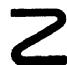
\includegraphics[keepaspectratio]{images/part001_5df2d3a1.jpg}}

Theorem 1 (no. 1) and Corollary 2 of Theorem 2 (no. 4) do not extend to locally compact spaces which are not compact.

For example, in an infinite discrete space X, the filter consisting of those sets which contain a given point \(x \in X\) and have a finite complement has x as its only cluster point but does not converge to x. Since any mapping f of X into a Hausdorff space \(X'\) is continuous, the image under f of an arbitrary subset of X (which is closed in X, since X is discrete) will not in general be a closed subset of \(X'\) .

The proposition corresponding to Theorem 3 of no. 5 is the following:

PROPOSITION 14. a) Let \((\mathbf{X}_{\iota})_{\iota \in I}\) be a family of locally compact spaces such that \(\mathbf{X}_{\iota}\) is compact for all but a finite number of indices. Then the product space \(\mathbf{X} = \prod_{\iota \in I} \mathbf{X}_{\iota}\) is locally compact.

\begin{enumerate}
\def\labelenumi{\alph{enumi})}
\setcounter{enumi}{1}
\item
  Conversely, if the product of a family \((\mathbf{X}_{\iota})_{\iota\in I}\) of non-empty topological spaces is locally compact, then the factors \(\mathbf{X}_{\iota}\) are compact for all but a finite number of indices, and the factors which are not compact are locally compact.
\item
  Let \(x = (x_{\iota})\) be a point of \(X\) . For each index \(\iota \in I\) such that \(X_{\iota}\) is locally compact but not compact, let \(V_{\iota}\) be a compact neighbourhood of \(x_{\iota}\) in \(X_{\iota}\) , and for all other indices \(\iota\) put \(V_{\iota} = X_{\iota}\) . Then \(\prod_{\iota \in I} V_{\iota}\) is a compact neighbourhood of \(x\) in \(X\) (no. 5, Theorem 3). Also \(X\) is Hausdorff by § 8, no. 2, Proposition 7, and is therefore locally compact.
\item
  If \(X = \prod_{\iota \in I} X_{\iota}\) is locally compact and the \(X_{\iota}\) non-empty, then each of the \(X_{\iota}\) is homeomorphic to a closed subspace of \(X\) (§ 4, no. 2, Proposition 4 and § 4, no. 3, Corollary to Proposition 7), hence locally compact by Proposition 13. Let \(a = (a_{\iota})\) be a point of \(X\) and let \(V\) be a compact neighbourhood of \(a\) ; since we have \(pr_{\iota}V = X_{\iota}\) for all but a finite number of indices (§ 4, no. 1), it follows from no. 4, Corollary 1 to Theorem 2, that the \(X_{\iota}\) are compact except for a finite number of indices.
\end{enumerate}

